% K80 model of evolution.
% A <--> G 	purines
% ^\   / ^
% |  X   |
% v/   \ v
% C <--> T	pyrimidines
%
% $ pdflatex k80
% $ pdf2svg k80.pdf k80.svg

\documentclass[11pt,tikz,border=2pt]{standalone}
\usepackage{tikz}
\usetikzlibrary{arrows}
\begin{document}
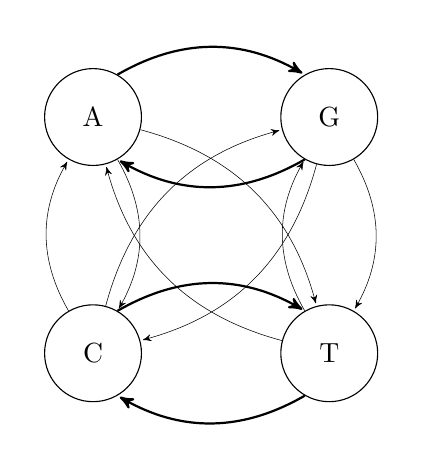
\begin{tikzpicture}[->,>=stealth',shorten >=1pt,auto,node distance=3cm,
		main node/.style={circle,draw,minimum size=35pt},
		invis node/.style={circle,minimum size=35pt}]
	\node[main node] (0) {A};
	\node[main node] (1) [right of=0] {G};
	\node[main node] (2) [below of=0] {C};
	\node[main node] (3) [right of=2] {T};
	%
	% Thick lines between purines A and G.
	\path[thick]
		(0.60) edge [bend left] node {} (1.120)
		(1.240) edge [bend left] node {} (0.300);
	%
	% Thick lines between pyrimidines C and T.
	\path[thick]
		(2.60) edge [bend left] node {} (3.120)
		(3.240) edge [bend left] node {} (2.300);
	%
	% Thin lines connecting a purine to a pyrimidine.
	\path[very thin]
		(0.300) edge [bend left] node {} (2.60)
		(2.120) edge [bend left] node {} (0.240);
	\path[very thin]
		(1.300) edge [bend left] node {} (3.60)
		(3.120) edge [bend left] node {} (1.240);
	\path[very thin]
		(0) edge [bend left] node {} (3)
		(3) edge [bend left] node {} (0);
	\path[very thin]
		(1) edge [bend left] node {} (2)
		(2) edge [bend left] node {} (1);


	%\path[]
		%(0.60) edge [bend left] node {$\lambda_0$} (1.120)
		%(1.60) edge [bend left] node {$\lambda_1$} (2.120)
		%(2.60) edge [bend left] node {} (3.120)
		%(3.60) edge [bend left] node {} (4.120)
		%(4.60) edge [bend left] node {$\lambda_{n-1}$} (5.120)
		%(5.60) edge [bend left] node {$\lambda_{n}$} (6.120)
		%(6.60) edge [bend left] node {} (7.120);
	%\path[]
		%(7.240) edge [bend left] node {} (6.300)
		%(6.240) edge [bend left] node {$\mu_{n+1}$} (5.300)
		%(5.240) edge [bend left] node {$\mu_{n}$} (4.300)
		%(4.240) edge [bend left] node {} (3.300)
		%(3.240) edge [bend left] node {} (2.300)
		%(2.240) edge [bend left] node {$\mu_2$} (1.300)
		%(1.240) edge [bend left] node {$\mu_1$} (0.300);
\end{tikzpicture}
\end{document}
